\documentclass{article}
\usepackage[utf8]{inputenc}
\usepackage{amsmath}
\usepackage{amssymb}
\usepackage{amsthm}
\usepackage{float}
\usepackage[colorlinks=true]{hyperref}
\usepackage{parskip}
\usepackage{ upgreek }
\usepackage{tikz}
\usetikzlibrary{arrows,automata}
\usepackage{fancyhdr}
\usepackage{pgfplots}
\usepackage{mathtools}

\usepackage[a4paper, total={6in, 8in}]{geometry}

\renewcommand{\vec}[1]{\mathbf{#1}}


\author{Elsie Mestl}
\date{\today}
\title{Mandatory Assignment 1 \\ mat2410 - Introduction to Complex analysis}


\pagestyle{fancy}
\lhead{Oblig 1. \quad mat2410-Introduction to Complex analysis}
\rhead{Elsie Mestl}

\begin{document}


\maketitle


\section*{Exercise 1}
\subsection*{a)}

% Find all roots of \[z^6 = \frac{1+ i}{\sqrt{3}+i}\]
Start by writing the formula to cartesian form
\[
\frac{1+ i}{\sqrt{3}+i} = \frac{(1+ i)(\sqrt{3}-i)}{(\sqrt{3}+i)(\sqrt{3}-i)} = \frac{\sqrt{3}+1 + i(\sqrt{3} -1)}{4}
\]

Rewrite to polar cordinates:
\begin{align*}
  r &= \sqrt{\left(\frac{\sqrt{3}+1}{4}\right)^2 + \left(\frac{\sqrt{3}-1}{4}\right)^2}
  &&\theta = \cos^{-1}\left(\frac{\frac{\sqrt{3}+1}{4}}{\frac{\sqrt{2}}{2}} \right)  = \cos^{-1}\left(\frac{\sqrt{3} +1}{2\sqrt{2}}\right)\\
  &= \sqrt{\frac{3 + 2\sqrt{3} + 1 + 3 -2\sqrt{3} +1}{16}}
  &&\theta = \sin^{-1}\left(\frac{\frac{\sqrt{3}-1}{4}}{\frac{\sqrt{2}}{2}} \right)  = \sin^{-1}\left(\frac{\sqrt{3} -1}{2\sqrt{2}}\right)
  \\
  &= \sqrt{\frac{1}{2}} = \frac{\sqrt{2}}{2}
  &&\theta = \frac{\pi}{12} \\
  \ \\
  \intertext{the roots are
  :} \\
  z^6 &= \frac{\sqrt{2}}{2}e^{i\left(\frac{\pi}{12} + 2\pi m\right)}  \implies z= \frac{\sqrt[\leftroot{3}12]{2^{11}}}{2}e^{i\left(\frac{\pi}{72} + \frac{\pi m}{3}\right)}, \qquad &&m = 0,1,2,3,4,5
\end{align*}


\subsection*{b)}
Can not use the same strategy as before because $\theta$ is not exact.
But what we can do is complete the square and get:
\begin{align*}
  \left(7 + 24i\right)^{\frac{1}{2}} = \left(7 + 9 -9 + 24i\right)^{\frac{1}{2}} =  \left(16 - 9 + 24i\right)^{\frac{1}{2}} =  \left(16  +9i^2 + 24i\right)^{\frac{1}{2}}= \left(4 + 3i\right)
\end{align*}
The other solution is rotated $\pi$ around the unit circle and the solutions are thus:

\[4 + 3i, \quad -4 -3i\]




\subsection*{c)}
\[\{z~|~ z^2 + \overline{z}^2 = 2\} = \{z~ | ~ x^2 + 2ixy - y^2 + x^2 -2ixy -y^2 = 2\} = \{z ~| ~ x^2 -y^2 = 1\}\]

Is the formula of a hyperbola and gives the following plot.\\
\pgfplotsset{every axis/.append style={
    axis x line=middle,    % put the x axis in the middle
    axis y line=middle,    % put the y axis in the middle
    axis line style={<->}, % arrows on the axis
    xlabel={$x$},          % default put x on x-axis
    ylabel={$y$},          % default put y on y-axis
}}

% arrows as stealth fighters
\tikzset{>=stealth}
\begin{center}
  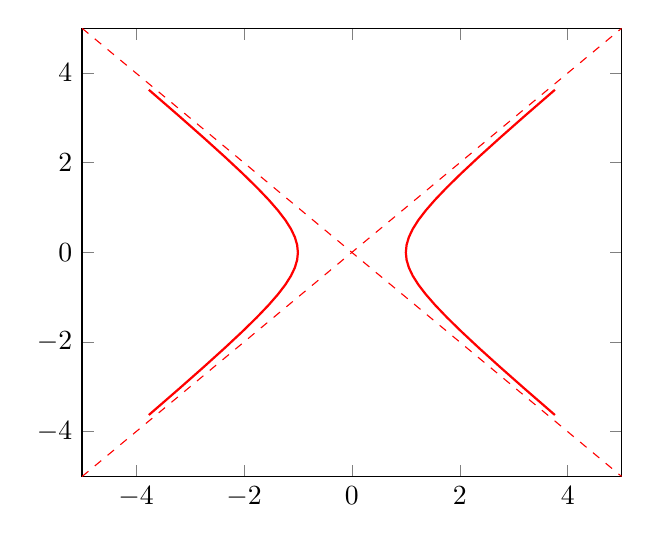
\begin{tikzpicture}
    \begin{axis}[
        xmin=-5,xmax=5,
        ymin=-5,ymax=5]
      \addplot [red,thick,domain=-2:2] ({cosh(x)}, {sinh(x)});
      \addplot [red,thick,domain=-2:2] ({-cosh(x)}, {sinh(x)});
      \addplot[red,dashed] expression {x};
      \addplot[red,dashed] expression {-x};
    \end{axis}

  \end{tikzpicture}
\end{center}





\subsection*{d)}

% Find a solution for

% \[z^2 -(1+i) z + \frac{i}{4} = 0\]

Insert into the bc-formula and get:

\begin{align*}
  z &= \frac{1 +i}{2} \pm \sqrt{\left(\frac{1 + i}{2}\right)^2 - \frac{i}{4}} = \frac{1 +i}{2} \pm \sqrt{\frac{i}{2} - \frac{i}{4}} = \frac{1 +i}{2} \pm \sqrt{\frac{i}{4}}
  \\
  \intertext{Rewrite the terms separately to polar coordinates}\\
  &= \frac{\sqrt{2}}{2}e^{i\frac{\pi}{4}} \pm \sqrt{\frac{1}{4}e^{i\frac{\pi}{2}}} = \frac{\sqrt{2}}{2}e^{i\frac{\pi}{4}} \pm \frac{1}{2}e^{i\frac{\pi}{4}}  = \frac{e^{i\frac{\pi}{4}}}{2}(\sqrt{2} \pm 1)\\
\end{align*}


\subsection*{e)}
$|f(z_1)-f(z_2)| = |\alpha z_1 + \beta - \alpha z_2 - \beta| = |\alpha(z_1 - z_2)|= |\alpha||z_1 - z_2|$\\
From this we can easily see that if $|\alpha| = 1$ then $|f(z_1) - f(z_2)| = |z_1 -z_2|$



\section*{Exercise 2}
\subsection*{a)}
Show that if U and V are convex then U $\cap$ V  is convex.

\begin{proof}[\unskip \nopunct]
  Let U and V be convex sets.
  And let $z_1, z_2$ be two arbitary points in U $\cap$ V. Need to show that there exists a straight line from $z_1$ to $z_2$ that lies in U $\cap$ V.

  But since $z_1, z_2 \in$ U $\cap$ V then $z_1, z_2 \in$ U, $z_1, z_2 \in$ V and since U and V are convex sets, that is there is a straight line between the points where the line itself lies in the set, i.e. for $t\in[0,1]$:
  \[tz_1 + (1-t)z_2 \in \text{U}, \quad tz_1 + (1-t)z_2 \in \text{V}\]

  This implies that
  \[tz_1 + (1-t)z_2 \in \text{U} \cap \text{V}\]

  And we have that U $\cap$ V is convex.

\end{proof}



\subsection*{b)}
Show that if U is convex then U $\cup \, \partial$U is convex.

Let $z_1, z_2$ bet two arbitary points in U$\cup \, \partial$U and U a convex set. Then there exists two sequences $\{w_n\}, \{v_n\} \subset$ U that converge respectly to $z_1$ and $z_2$.

And since $\{w_n\}, \{v_n\} \subset$ U we know that for every $i, j$ there is a straight line between $w_i$ and $v_j$. i.e.
\[tw_i +(1-t)v_j \in \text{U} \]
And as $\{w_n\} \rightarrow r_1$ and $\{v_n\} \rightarrow r_2$  
\[tr_1 +(1-t)r_2 \in \text{U$\cup \, \partial$U} \]
as $n \rightarrow \infty$.

Thereby we have that U$\cup \, \partial$U is a convex set

%%%%%%%%%%%%%%%%%%%%%%%%%%%%%%%%%%%%%%%
\newpage
\section*{Exercise 3}
\[\left<z, w\right> = \operatorname{Re}(z\overline{w}), \quad z = a +ib, \, w = x +iy\]

\subsection*{a)}
\subsubsection*{Show that $|z| = \left<r, r\right>^{1/2}$}
\begin{proof}[\unskip\nopunct]
  \[\left<r, r\right>^{1/2} = \operatorname{Re}(z\overline{z})^{1/2} = \operatorname{Re}((a + ib)(a -ib))^{1/2}=\operatorname{Re}(a^2 + b^2)^{1/2} = (a^2 + b^2)^{1/2} = |z|\]
\end{proof}


\subsubsection*{Show the Cauchy-Schwartz ineqiuality i.e. \\
Show that $|\left<z, w\right>| \leq |z||w|$}
\begin{proof}[\unskip\nopunct]
  Uses polar coordinates
  \begin{align*}|\left<z, w\right>| &= |\operatorname{Re}(z\overline{w})| =  |\operatorname{Re}(r_ze^{i\text{arg(z)}}r_we^{-i\text{arg(w)}})| =|\operatorname{Re}(r_zr_we^{i(\text{arg(z)- arg(w)})})| = |r_zr_w\cos(\text{arg(w) - arg(w)})| \\
    &\leq |r_zr_w| = |r_z||r_w| = ||z||||w|| = |z||w|
  \end{align*}
\end{proof}



\subsubsection*{Show the triangle inequality i.e.\\
  Show $|z + w| \leq |z| + |w| $}

\begin{proof}[\unskip\nopunct]
  \begin{align*}|z + w| &= \left<z + w, z+ w\right>^{1/2} = \operatorname{Re}((z+w)\overline{(z+w)})^{1/2} = \operatorname{Re}((z+w)(\overline{z}+\overline{w}))^{1/2} \\
    &= \operatorname{Re}(z\overline{z} + w\overline{w} + z\overline{w} + \overline{z}w)^{1/2} \\
    &= \operatorname{Re}(r_z^2e^{i\text{arg(z)} - i\text{arg(z)}} + r_w^2 e^{i\text{arg(w)} -i\text{arg(w)}} + r_zr_we^{i(\text{arg(z) - arg(w)})} + r_zr_we^{-i(\text{arg(z)-arg(w)} )})^{1/2} \\
    &=\operatorname{Re}(r^2_z + r^2_w + 2r_zr_w\cos(\text{arg(z) - arg(w)}))^{1/2} \leq (r^2_w + r^2_z + 2r_wr_z)^{1/2} = ((r_w + r_z)^2)^{1/2} = |z| + |w|
  \end{align*}
\end{proof}



\subsection*{b)}
\begin{proof}[\unskip\nopunct]

  Need to show the implication in both directions:


  $\pmb{\Rightarrow}$ Show that if $\left<z, w \right> = 0 $ then  $z/w$ is pure imaginary:

  That $\left<z, w \right> = 0 $ implies that $\operatorname{Re}(z\overline{w}) = 0$ wich means $\operatorname{Re}(z)\operatorname{Re}(w) + \operatorname{Im}(z)\operatorname{Im}(w) = 0$

  \begin{align*}z/w &= \frac{\operatorname{Re}(z) + i\operatorname{Im}(z)}{\operatorname{Re}(w) + i\operatorname{Im}(w)} = \frac{(\operatorname{Re}(z) + i\operatorname{Im}(z))(\operatorname{Re}(w) - i\operatorname{Im}(w))}{\operatorname{Re}(w)^2 + Im(w)^2} \\&= \frac{(\operatorname{Re}(z)\operatorname{Re}(w) + \operatorname{Im}(z)\operatorname{Im}(w) + i(\operatorname{Re}(w)\operatorname{Im}(z) - i\operatorname{Im}(w)\operatorname{Re}(z))}{\operatorname{Re}(w)^2 + \operatorname{Im}(w)^2} \\
    &= \frac{i(\operatorname{Re}(w)\operatorname{Im}(z) - i\operatorname{Im}(w)\operatorname{Re}(z))}{\operatorname{Re}(w)^2 + \operatorname{Im}(w)^2}
  \end{align*}

  And we have that $z/w$ has no real part


  $\pmb{\Leftarrow}$ Show that if $z/w$ is pure imaginary then $\left<z, w \right> = 0$

  That $z/w$ is pure imaginary means that $\operatorname{Re}(z)\operatorname{Re}(w) + \operatorname{Im}(z)\operatorname{Im}(w) = 0$
  \[\left<z,w \right> = \operatorname{Re}(z\overline{w}) = \operatorname{Re}(z)\operatorname{Re}(w) + \operatorname{Im}(z)\operatorname{Im}(w) \]

  Therfore $\left<z,w \right>$ must be equal to 0 if $z/w$ is pure imaginary.

  And since both implications hold, we know the statement to be true

\end{proof}



\section*{Exercise 4}
\subsection*{a)}
\[\lim_{n\to\infty} \left(\frac{i}{2}\right)^n  =\lim_{n\to\infty} \left(\frac{e^{i\pi/2}}{2}\right)^n = \lim_{n\to\infty} \frac{e^{in\pi/2}}{2^n}  = 0, \qquad \text{Since $e^{in\pi/2}$ is periodic} \]


\subsection*{b)}

\[\lim_{z\to\infty} \frac{z^2 + 1}{z + i} = \lim_{z\to\infty} \frac{(z + i)(z-i)}{(z + i)} = \lim_{z\to\infty} z-i =\infty \]



\subsection*{c)}
\[\lim_{n\to\infty} \left(1+ \frac{i}{n}\right)^{n\pi} = \lim_{n\to\infty}e^{\ln\left(\left(1+ \frac{i}{n}\right)^{n\pi}\right)}
=  \lim_{n\to\infty}e^{n\pi\cdot\ln\left(1+ \frac{i}{n}\right)} = \lim_{n\to\infty}e^{\frac{\pi\ln\left(1+ \frac{i}{n}\right)}{1/n}}
= \lim_{n\to\infty}e^{\pi\frac{\frac{\frac{-i}{n^2}}{1+ \frac{i}{n}}}{\frac{-1}{n^2}}} = \lim_{n\to\infty}e^{\pi\frac{i}{1+ \frac{i}{n}}} = e^{i\pi}
\]



\section*{Exercise 5}
\subsection*{a)}
\subsubsection*{i.}
\begin{align*}
\frac{\partial f}{\partial z} &= \frac{\partial z^2}{\partial z}
=\frac{1}{2}\left(\frac{\partial}{\partial x} (x^2+2ixy -y^2)  - i \frac{\partial}{\partial y} (x^2+2ixy -y^2) \right) = \frac{1}{2}\left(\frac{\partial x^2 - y^2}{\partial x} + i\frac{\partial 2xy}{\partial x} - i\frac{\partial x^2 -y^2}{\partial y} + \frac{\partial 2xy}{\partial y}\right) \\
  &= \frac{1}{2}(2x + i2y + i2y + 2x) = 2x + 2iy = 2z
\end{align*}

\begin{align*}\frac{\partial f}{\partial \overline{z}} &= \frac{\partial z^2}{\partial \overline{z}} =\frac{1}{2}\left(\frac{\partial}{\partial x} (x^2+2ixy -y^2)  + i \frac{\partial}{\partial y} (x^2+2ixy -y^2) \right) = \frac{1}{2}\left(\frac{\partial x^2 - y^2}{\partial x} + i\frac{\partial 2xy}{\partial x} + i\frac{\partial x^2 -y^2}{\partial y} - \frac{\partial 2xy}{\partial y}\right) \\
  &= \frac{1}{2}(2x + i2y - i2y - 2x) = 0 \end{align*}


\subsubsection*{ii.}
\begin{align*}\frac{\partial f}{\partial z} &= \frac{\partial e^z}{\partial z} = \frac{1}{2}\left(\frac{\partial}{\partial x} (e^{x +iy})  - i \frac{\partial}{\partial y} (e^{x + iy}) \right) = \frac{1}{2}\left(\frac{\partial e^x\cos(y)}{\partial x} + i\frac{e^x\sin(y)}{\partial x} -i\frac{\partial e^x\cos(y)}{\partial y} + \frac{e^x\sin(y)}{\partial y}\right) \\
  &= \frac{1}{2}\left(e^x\cos(y) +ie^x\sin(y) +i e^x\sin(y) + e^x\cos(y) \right) = e^{x}\cos(y) + ie^x\sin(y) = e^x(e^{iy}) = e^{x+iy} = e^z \end{align*}

\begin{align*}\frac{\partial f}{\partial \overline{z}} &= \frac{\partial e^z}{\partial \overline{z}} = \frac{1}{2}\left(\frac{\partial}{\partial x} (e^{x +iy})  + i \frac{\partial}{\partial y} (e^{x + iy}) \right) = \frac{1}{2}\left(\frac{\partial e^x\cos(y)}{\partial x} + i\frac{e^x\sin(y)}{\partial x} + i\frac{\partial e^x\cos(y)}{\partial y} - \frac{e^x\sin(y)}{\partial y}\right) \\
  &= \frac{1}{2}\left(e^x\cos(y) +ie^x\sin(y) -i e^x\sin(y) - e^x\cos(y) \right) = 0 \end{align*}


\subsubsection*{iii.}
\begin{align*}\frac{\partial f}{\partial z} &= \frac{\partial |z|^2}{\partial z} =\frac{1}{2}\left(\frac{\partial}{\partial x} (x^2 + y^2)  - i \frac{\partial}{\partial y} (x^2 +y^2) \right) = x -iy = \overline{z}\end{align*}

\begin{align*}\frac{\partial f}{\partial \overline{z}} &= \frac{\partial |z|^2}{\partial \overline{z}} =\frac{1}{2}\left(\frac{\partial}{\partial x} (x^2 + y^2)  + i \frac{\partial}{\partial y} (x^2 +y^2) \right) = x + iy = z\end{align*}


  \subsubsection*{iv.}
  \[\frac{\partial f}{\partial z} = \frac{\partial \operatorname{Im}(z)}{\partial z} =\frac{1}{2}\left(\frac{\partial}{\partial x} (y)  - i \frac{\partial}{\partial y} (y) \right) = -i \]

  \[\frac{\partial f}{\partial \overline{z}} = \frac{\partial \operatorname{Im}(z)}{\partial \overline{z}} =\frac{1}{2}\left(\frac{\partial}{\partial x} (y)  + i \frac{\partial}{\partial y} (y) \right) = i \]


  \subsection*{b)}
  \subsubsection*{i}
  Have that:
  \begin{align*}
    \frac{\partial f}{\partial x} &= \frac{\partial u}{\partial x} + i\frac{\partial v}{\partial x}
    &\frac{\partial \overline{f}}{\partial x} = \frac{\partial u}{\partial x} - i\frac{\partial v}{\partial x}
  \end{align*}
  By summing the formulas we get
  \[
  \frac{\partial f}{\partial x} +\frac{\partial  \overline{f}}{x}= 2\frac{\partial u}{\partial x} \implies \frac{\partial u}{\partial x} = \frac{1}{2}\left(\frac{\partial f}{\partial x} + \frac{\partial \overline{f}}{\partial x}\right)
  \]


  Have that:
  \begin{align*}
    \frac{\partial f}{\partial y} &= \frac{\partial u}{\partial y} + i\frac{\partial v}{\partial y}
    &\frac{\partial \overline{f}}{\partial y} = \frac{\partial u}{\partial y} - i\frac{\partial v}{\partial y}
  \end{align*}
  By summing the formulas we get
  \[\frac{\partial f}{\partial y} + \frac{\partial \overline{f}}{\partial y} = 2\frac{\partial u}{\partial y} \implies \frac{\partial u}{\partial y} = \frac{1}{2}\left(\frac{\partial f}{\partial y} + \frac{\partial \overline{f}}{\partial y}\right)\]

  \subsubsection*{ii}
  By subtracting the formulas from above we get
  \[
  \frac{\partial f}{\partial x} - \frac{\partial  \overline{f}}{x}= 2i\frac{\partial v}{\partial x} \implies \frac{\partial v}{\partial x} = \frac{1}{2i}\left(\frac{\partial f}{\partial x} - \frac{\partial \overline{f}}{\partial x}\right)
  \]

  \[
  \frac{\partial f}{\partial y} - \frac{\partial  \overline{f}}{y}= 2i\frac{\partial v}{\partial y} \implies \frac{\partial v}{\partial y} = \frac{1}{2i}\left(\frac{\partial f}{\partial y} - \frac{\partial \overline{f}}{\partial y}\right)
  \]


  \subsubsection*{iii}
  Have that:
  \begin{align*}
    \frac{\partial f}{\partial z} &= \frac{1}{2}\left(\frac{\partial f}{\partial x} - i\frac{\partial f}{\partial y}\right)
    &\frac{\partial f}{\partial \overline{z}} = \frac{1}{2}\left(\frac{\partial f}{\partial x} + i\frac{\partial f}{\partial y}\right)
  \end{align*}

  Summing the formulas we get

  \[\frac{\partial f}{\partial z} + \frac{\partial f}{\partial \overline{z}} = \frac{1}{2}\left(2\frac{\partial f}{\partial x}\right) \implies \frac{\partial f}{\partial x} = \frac{\partial f}{\partial z} + \frac{\partial f}{\partial \overline{z}}\]

  Subtracting the formulas we get

  \[\frac{\partial f}{\partial z} - \frac{\partial f}{\partial \overline{z}} = \frac{1}{2}\left(-2i\frac{\partial f}{\partial y}\right) \implies \frac{\partial f}{\partial y} = i\left(\frac{\partial f}{\partial z} - \frac{\partial f}{\partial \overline{z}}\right)\]


  \subsection*{c)}

  Let $D(f)= \frac{\partial f}{\partial z}$ or $D(f)= \frac{\partial f}{\partial \overline{z}}$. Will show all the properties with $D(f) = \frac{\partial f}{\partial z}$ but the argument is the same for $D(f)= \frac{\partial f}{\partial \overline{z}}$ but with a change in signs.

  \subsubsection*{Show that $D(\alpha f + \beta g) = \alpha D(f) + \beta D(g)$ for any complex constant $\alpha, \beta$}

  \begin{proof}[\unskip\nopunct]
    \begin{align*}D(\alpha f + \beta g) &= \frac{\partial (\alpha f + \beta g)}{\partial z} = \frac{1}{2}\left(\frac{\partial (\alpha f + \beta g)}{\partial x} - i\frac{\partial (\alpha f + \beta g)}{\partial y} \right)  \\
      &=  \frac{1}{2}\left(\frac{\partial (\alpha u_f + \beta u_g)}{\partial x}  + i \frac{\partial (\alpha v_f + \beta v_g)}{\partial x} - i\frac{\partial (\alpha u_f + \beta u_g)}{\partial y}  + \frac{\partial (\alpha v_f + \beta v_g)}{\partial y} \right)\\
      \intertext{Since u, v are real valued functions we allready know the rule holds for them, and get:}
      &= \frac{1}{2}\left(\frac{\alpha\partial u_f + \beta\partial u_g}{\partial x} + i\frac{\alpha\partial v_f + \beta\partial v_g}{\partial x}  -i\frac{\alpha\partial u_f + \beta\partial u_g}{\partial y} + \frac{\alpha\partial v_f + \beta\partial v_g}{\partial y}\right) \\
      &=\frac{1}{2}\left(\alpha\frac{\partial f}{\partial x} + \beta\frac{\partial g}{\partial x} -i\left( \alpha\frac{\partial f}{\partial y} + \beta\frac{\partial g}{\partial y} \right)\right) = \alpha \frac{\partial f}{\partial z} + \beta \frac{\partial g}{\partial z} = \alpha D(f) + \beta D(g)
    \end{align*}
  \end{proof}

  \subsubsection*{Show that the Leibnitz rule holds:}

  \begin{proof}[\unskip \nopunct]
    \begin{align*}
      D(fg)  &= \frac{\partial (fg)}{\partial z} = \frac{1}{2}\left(\frac{\partial fg}{\partial x} - i\frac{\partial fg}{\partial y} \right) \\
      &= \frac{1}{2}\left(\frac{\partial (u_fu_g - v_fv_g)}{\partial x} + i\frac{\partial (u_fv_g + u_gv_f)}{\partial x} - i\frac{\partial (u_fu_g - v_fv_g)}{\partial y} + \frac{\partial (u_fv_g + u_gv_f)}{\partial y} \right) \\
      \intertext{Since u,v are real valued functions we know the Leibnitz rule holds}
      &= \frac{1}{2}\left(u_f\frac{\partial u_g}{\partial x} + u_g\frac{\partial u_f}{\partial x} - \left(v_f\frac{\partial v_g}{\partial x} + v_g\frac{\partial v_f}{\partial x}\right) + (\cdots) + u_f\frac{\partial v_g}{\partial y} + v_g\frac{\partial u_f}{\partial y} + \left(v_f\frac{\partial u_g}{\partial y} + u_g\frac{\partial v_f}{\partial y} \right)\right) \\
      &= \frac{1}{2}\left(u_f\frac{\partial g}{\partial x} + u_g\frac{\partial f}{\partial x}  + i\left( v_f\frac{\partial g}{\partial x} + v_g\frac{\partial f}{\partial x}\right)  -i\left( u_f\frac{\partial g}{\partial y} + u_g\frac{\partial f}{\partial y}  + i\left( v_f\frac{\partial g}{\partial y} + v_g\frac{\partial f}{\partial y}\right)\right)\right) \\
      &= u_f\frac{\partial g}{\partial z} + u_g\frac{\partial f}{\partial z} + i\left(v_f\frac{\partial g}{\partial z} + v_g\frac{\partial f}{\partial z}\right) = f\frac{\partial g}{\partial x} + g\frac{\partial f}{\partial z} = fD(g) + gD(f)
    \end{align*}
  \end{proof}


 \subsubsection*{Show that the quotient rule holds:}
  \begin{proof}[\unskip \nopunct]
    \begin{align*}
      D(\frac{f}{g})  &= \frac{\partial (f/g)}{\partial z} = \frac{\partial fg^{-1}}{\partial z} = f\frac{\partial g^{-1}}{\partial z} + g^{-1}\frac{\partial f}{\partial z} = \frac{f}{2}\left(\frac{\partial \frac{u_g - iv_g}{u^2_g + v^2_g}}{\partial x} - i\frac{\partial \frac{u_g - iv_g}{u^2_g + v^2_g}}{\partial y} \right)+ \frac{1}{g}\frac{\partial f}{\partial z}\\
      &= \frac{f}{2}\left(\frac{\partial\frac{u_g}{u^2_g + v^2_g}}{\partial x} -i \frac{\partial \frac{v_g}{u^2_g + v^2_g}}{\partial x} -i\left( \frac{\partial\frac{u_g}{u^2_g + v^2_g}}{\partial y} -i \frac{\partial \frac{v_g}{u^2_g + v^2_g}}{\partial y}\right)\right)+ \frac{gD(f)}{g^2} \\
      \intertext{Know the quotient rule holds for real valued functions. Get:}
      &= \frac{g D(f)}{g^2} + \frac{f}{2}\left( \frac{u^2_g + v^2_g}{(u^2_g + v^2_g)^2}\frac{\partial u_g}{\partial x} -\frac{u_g}{(u^2_g + v^2_g)^2}\frac{\partial u^2_g + v^2_g}{\partial x} -i\left(\frac{u^2_g + v^2_g}{(u^2_g + v^2_g)^2}\frac{\partial v_g}{\partial x} -\frac{v_g}{(u^2_g + v^2_g)^2}\frac{\partial u^2_g + v^2_g}{\partial x}\right)\right) \\ &\qquad -i\frac{f}{2}\left(\frac{u^2_g + v^2_g}{(u^2_g + v^2_g)^2}\frac{\partial u_g}{\partial y} -\frac{u_g}{(u^2_g + v^2_g)^2}\frac{\partial u^2_g + v^2_g}{\partial y} -i\left(\frac{u^2_g + v^2_g}{(u^2_g + v^2_g)^2}\frac{\partial v_g}{\partial y} -\frac{v_g}{(u^2_g + v^2_g)^2}\frac{\partial u^2_g + v^2_g}{\partial y}\right)\right) \\
      &= \frac{g D(f)}{g^2} + \frac{f}{2|g|^4}\left( (u^2_g + v^2_g)\frac{\partial u_g}{\partial x} + (-u_g + iv_g)\frac{\partial u^2_g + v^2_g}{\partial x} -i(u^2_g + v^2_g)\frac{\partial v_g}{\partial x}\right) \\ &\qquad -i\frac{f}{2|g|^4}\left((u^2_g + v^2_g)\frac{\partial u_g}{\partial y} +(-u_g + iv_g)\frac{\partial u^2_g + v^2_g}{\partial y} -i(u^2_g + v^2_g)\frac{\partial v_g}{\partial y}\right)\\
      &= \frac{g D(f)}{g^2} + \frac{f}{2|g|^4}\left( (u^2_g + v^2_g)\frac{\partial u_g}{\partial x} + (-u_g + iv_g)\left(2u_g\frac{\partial u_g}{\partial x} + 2v_g\frac{\partial v_g}{\partial x}\right) -i(u^2_g + v^2_g)\frac{\partial v_g}{\partial x}\right) \\ &\qquad -i\frac{f}{2|g|^4}\left((u^2_g + v^2_g)\frac{\partial u_g}{\partial y} +(-u_g + iv_g)\left(2u_g\frac{\partial u_g}{\partial y} + 2v_g\frac{\partial v_g}{\partial y}\right) -i(u^2_g + v^2_g)\frac{\partial v_g}{\partial y}\right)\\
      &=\frac{g D(f)}{g^2} + \frac{f}{2|g|^4}\left(\frac{\partial u_g}{\partial x}(u_g^2 + v_g^2 - 2u_g^2 + 2iu_gv_g) + i\frac{\partial v_g}{\partial x}(2iv_gu_g + 2v_g^2 -u_g^2 - v_g^2)\right) \\ &\qquad -i\frac{f}{2|g|^4}\left(\frac{\partial u_g}{\partial y}(u_g^2 + v_g^2 - 2u_g^2 + 2iu_gv_g) + i\frac{\partial v_g}{\partial y}(2iv_gu_g + 2v_g^2 -u_g^2 - v_g^2)\right)\\
      &= \frac{g D(f)}{g^2} + \frac{f}{2|g|^4}\left(\frac{\partial u_g}{\partial x}(v_g +iu_g)^2 + i\frac{\partial v_g}{\partial x}(v_g +iu_g)^2 -i\left(\frac{\partial u_g}{\partial y}(v_g +iu_g)^2 + i\frac{\partial v_g}{\partial y}(v_g +iu_g)^2\right)\right)\\
      &= \frac{g D(f)}{g^2} + \frac{f}{2|g|^4}\left(\frac{\partial g}{\partial x}(i(u_g - iv_g))^2 -i\frac{\partial g}{\partial y}(i(u_g - iv_g))^2 \right) = \frac{g D(f)}{g^2} + \frac{f}{2|g|^4}\left(\frac{\partial g}{\partial x}(i\overline{g})^2 - i\frac{\partial g}{\partial y}(i\overline{g})^2\right) \\
      &=\frac{g D(f)}{g^2} + \frac{f(i\overline{g})^2}{|g|^4}\left(\frac{\partial g}{\partial z}\right)  =  \frac{g D(f)}{g^2} + \frac{-f\overline{g}^2}{|g|^4}D(g) =  \frac{g D(f)}{g^2} + \frac{-f(r_ge^{-i\operatorname{Arg}(g)})^2}{r_g^4}D(g) \\
      &=  \frac{g D(f)}{g^2} + \frac{-f}{r_g^2e^{2i\operatorname{Arg}(g)}}D(g)  = \frac{g D(f) -fD(g)}{g^2}
    \end{align*}
  \end{proof}



  \subsection*{d)}
  \begin{proof}[\unskip\nopunct]
    $\pmb{\Rightarrow}$ Show that if $\frac{\partial f}{\partial \overline{z}} = 0$ then the Cauchy-Riemann equations hold


    \begin{align*}\frac{\partial f}{\partial \overline{z}} &= \frac{1}{2}\left(\frac{\partial f}{\partial x} + i\frac{\partial f}{\partial y}\right) = 0 \implies \frac{\partial f}{\partial x} = -i\frac{\partial f}{\partial y} \implies \frac{\partial u }{\partial x} + i \frac{\partial v }{\partial x} = -i\left(\frac{\partial u }{\partial y} + i\frac{\partial v }{\partial y}\right)\\
      &\implies \frac{\partial u }{\partial x} = \frac{\partial v}{\partial y}, \quad \frac{\partial v }{\partial x} = - \frac{\partial u }{\partial y}
    \end{align*}


    $\pmb{\Leftarrow}$ Show that if the Cauchy-Riemann equations hold then $\frac{\partial f}{\partial \overline{z}} = 0$
    Have that
    \begin{align*}
      \frac{\partial u }{\partial x} = \frac{\partial v}{\partial y}, \quad \frac{\partial v }{\partial x} = - \frac{\partial u }{\partial y}
    \end{align*}

    Then

    \begin{align*}
      \frac{\partial f}{\partial \overline{z}} &= \frac{1}{2}\left(\frac{\partial f}{\partial x} + i\frac{\partial f}{\partial y}\right) = \frac{1}{2}\left(\frac{\partial u}{\partial x} +  i\frac{\partial v}{\partial x} + i\frac{\partial u}{\partial y} - \frac{\partial v}{\partial y}\right) = \frac{1}{2}\left(\frac{\partial v}{\partial y} -  i\frac{\partial u}{\partial y} + i\frac{\partial u}{\partial y} - \frac{\partial v}{\partial y}\right) = 0
    \end{align*}


    Since both implications hold the statements are equivalent.

  \end{proof}
  
\begin{align*}\frac{\partial f}{\partial z} &= \frac{1}{2}\left(\frac{\partial f}{\partial x} - i\frac{\partial f}{\partial y}\right) = \frac{1}{2}\left(\frac{\partial u}{\partial x} +i\frac{\partial v}{\partial x}- i\frac{\partial u}{\partial y} + \frac{\partial v}{\partial y}\right)  = \frac{1}{2}\left(\frac{\partial u}{\partial x} + i\frac{\partial v}{\partial x} +  i\frac{\partial v}{\partial x} + \frac{\partial u}{\partial x}\right)  \\
  &=\frac{\partial u}{\partial x} + i\frac{\partial v}{\partial x} = \frac{\partial f}{\partial x} = \lim_{\Delta x \to 0} \frac{f(z + \Delta x) - f(z)}{\Delta x} = \lim_{\Delta z \to 0}\frac{f(z + \Delta z) - f(z)}{\Delta z} = f'(z) 
\end{align*}

Where at the last two steps we know the limit needs to be the same if we go along one or both axis.

\subsection*{e)}

Know that $f$ is analytic if and only if the Cauchy-Riemann equations hold. And know that the Cauchy-Riemann equations hold if and only if $\frac{\partial f}{\partial \overline{z}} = 0$. This means that $f$ is analytic if and only if $\frac{\partial f}{\partial \overline{z}} = 0$

\[\frac{\partial f}{\partial \overline{z}} = \frac{1}{2}\left(\frac{\partial f}{\partial x} + i\frac{\partial f}{\partial y}\right) = \frac{1}{2}\left(\frac{\partial u}{\partial x} + i\frac{\partial v}{\partial x} + i\frac{\partial u}{\partial y} - \frac{\partial v}{\partial y}\right) \]
  \subsubsection*{i.}

  \begin{align*}
    f(z) = \operatorname{Re}(z)\\
    \ \\
    &\frac{\partial u}{\partial x} = \frac{\partial \operatorname{Re}(z)}{\partial x} = \frac{\partial x}{\partial x} = 1
    & \frac{\partial v}{\partial y} = \frac{\partial 0}{\partial y} = 0
    \\
    &\frac{\partial u}{\partial y} = \frac{\partial \operatorname{Re}(z)}{\partial y}  = \frac{\partial x}{\partial x} = 0
    & \frac{\partial v}{\partial x} = \frac{\partial 0}{\partial x} = 0
  \end{align*}
    
  The Cauchy-Riemann equations do not hold and Re(z) is therefore not analytic

  \subsubsection*{ii.}
  \begin{align*}
    f(z) = (x^2 - y^2)+ 2xyi = z^2\\
  \end{align*}

  Know from exercise 5ai that $\frac{\partial z^2}{\partial \overline{z}} = 0$ and $f$ is therefore analytic 


  \subsubsection*{iii.}
  \begin{align*}
    &f(z) = e^{iy} = \cos(y) + i\sin(y)\\
    \ \\
   &\frac{\partial u}{\partial x} = \frac{\partial \cos(y)}{\partial x} = 0
    && \frac{\partial v}{\partial y} = \frac{\partial \sin(y)}{\partial y} = \cos(y)
    \\
    &\frac{\partial u}{\partial y} = \frac{\partial \cos(y)}{\partial y}  = -\sin(y)
    && \frac{\partial v}{\partial x} = \frac{\partial \sin(y)}{\partial x} = 0
  \end{align*}

  The Cauchy-Riemann equations do not hold, and $f$ is not analytic


  \subsubsection*{iv.}
  \begin{align*}
    f(z) &= z(z + \overline{z}^2) = z^2 +|z|^2\overline{z} = x^2 +2ixy - y^2 +&&(x^2 + y^2)(x + iy) =  x^3 + x^2 +y^2x -y^2 + i(2xy + x^2y + y^3) \\
    \ \\
    &\frac{\partial u}{\partial x} = \frac{\partial (x^3 + x^2 +y^2x -y^2)}{\partial x} = 3x^2 + 2x
    && \frac{\partial v}{\partial y} = \frac{\partial (2xy + x^2y + y^3)}{\partial y} = 2x + x^2 + 3y^2
    \\
    &\frac{\partial u}{\partial y} = \frac{\partial x^3 + x^2 +y^2x -y^2}{\partial y}  = 2yx - 2y
    && \frac{\partial v}{\partial x} = \frac{\partial (2xy + x^2y + y^3)}{\partial x} = 2y +2xy
  \end{align*}

  Cauchy-Riemann doesn't hold so the function is not analytic




\pagebreak
  \section*{Exercise 6}
  Let \[f(z) =
  \begin{cases}
    \frac{x^3 - y^3}{x^2 + y^2} + i\frac{x^3 + y^3}{x^2 + y^2} & z \neq 0 \\
    0 & z = 0
  \end{cases}
  \]

  \subsection*{a)}
  \begin{proof}[\unskip \nopunct]
  For any $\epsilon >0$ there exists a $\delta >0$ such that when $|f(0) - f(w)| < \epsilon$ then $|0- w | = |w| < \delta$

  \begin{align*}
    |f(0) - f(w)| &= \left|-\left(  \frac{u^3 - v^3}{u^2 + v^2} + i\frac{u^3 + v^3}{u^2 + v^2}\right)\right| \leq \left| \frac{u^3 -v^3}{|w|^2}\right| + |i|\left| \frac{u^3 + v^3}{|w|^2}\right| \\ 
    &\leq  \frac{2(|u| +|v|)(u^2 +v^2)}{||w|^2|} + \frac{2(|u| + |v|)(u^2 + v^2)}{||w|^2|}\\
    &= \frac{4(|u| + |v|)|w|^2}{|w|^2} = 4(|u| + |v|) \leq 4(|w| + |w|) =  8|w| < 8\delta = 8\frac{\epsilon}{8} = \epsilon
  \end{align*}
By choosing $\delta = \epsilon/8$\\
And we have that $f$ is continuous at 0
  \end{proof}

  
  \subsection*{b)}
  Need to check the Cauchy-Riemann equations, for $z = 0$ this is trivial and the answer is yes. For $z \neq 0$ we get:

  \begin{align*}
    \frac{\partial u}{\partial x} &=\frac{\partial \left(\frac{x^3 - y^3}{x^2 + y^2}\right)}{\partial x} = \frac{3x^2(x^2 + y^2) - (x^3 - y^3)(2x)}{(x^2 + y^2)^2} = \frac{x^4 + 3x^2y^2 + 2xy^3}{(x^2 + y^2)^2}\\
        \frac{\partial v}{\partial y} &=\frac{\partial \left(\frac{x^3 + y^3}{x^2 + y^2}\right)}{\partial y} = \frac{3y^2(x^2 + y^2) - (x^3 + y^3)(2y)}{(x^2 + y^2)^2} = \frac{y^4 + 3x^2y^2 - 2x^3y}{(x^2 + y^2)^2} 
  \end{align*}

See that the Cauchy-Riemann equation $\frac{\partial u}{\partial x} = \frac{\partial v}{\partial y}$ does not hold. And have that $f$ is thereby not analytic

\end{document}
